%
%===============>>  Симонов Модуль 9 <<=============
%
\setmodule{9}

%BEGIN_FOLD % ====>>_____ Занятие 1 _____<<====
\begin{class}[number=1]
	\begin{listofex}
		\item Решите уравнения:
		\begin{tasks}(2)
			\task \( x^2+3x=4 \)
			\task \( \dfrac{5}{4}x^2+7x+9=0 \)
		\end{tasks}
		\item Решите уравнения:
		\begin{tasks}(2)
			\task \( \dfrac{1}{x^2}-\dfrac{1}{x}-6=0 \)
			\task \( \dfrac{1}{(x-1)^2}+\dfrac{2}{x-1}-3=0 \)
		\end{tasks}
		\item Решите уравнения:
		\begin{tasks}(2)
			\task \( \dfrac{2x^2+7x-4}{x^2-16}=1 \)
			\task \( \dfrac{2x^2+3x-2}{x^2-4}=1 \)
		\end{tasks}
		\item Решите уравнения:
		\begin{tasks}(2)
			\task \( x^2-2x+\sqrt{3-x}=\sqrt{3-x}+8 \)
			\task \( x^2-3x+\sqrt{6-x}=\sqrt{6-x}+28 \)
		\end{tasks}
		\item Решите уравнение:
		\[x^6=(6x-5)^3\]
	\end{listofex}
\end{class}
%END_FOLD

%BEGIN_FOLD % ====>>_____ Занятие 2 _____<<====
\begin{class}[number=2]
	\begin{listofex}
	\item .
	\end{listofex}
\end{class}
%END_FOLD

%BEGIN_FOLD % ====>>_ Домашняя работа 1 _<<====
\begin{homework}[number=1]
	\begin{listofex}
		\item Найдите значение выражения: \(\dfrac{9,4}{4,1+5,3}\).
		\item О числах \( a \), \( b\), \( c \) и \( d \) известно, что \( a<b \), \( b=c \), \( d>c \). Сравнитe числа \( d \) и \( a \).
		\begin{tasks}(4)
			\task \( d=a \)
			\task \( d>a \)
			\task \( d<a \)
			\task Сравнить невозможно.
		\end{tasks}
		\item Найдите значение выражения \( \sqrt{7\cdot12}\cdot\sqrt{21} \).
		\item Решите уравнениe: \(\dfrac{x}{4}+x=4\).
		\item Миша с папой решили покататься на колесе обозрения. Всего на колесе пятнадцать кабинок, из них \( 2 \) --- синие, \( 10 \) --- зеленые, остальные  --- красные. Кабинки по очереди подходят к платформе для посадки. Найдите вероятность того, что Миша прокатится в красной кабинке.
		\item Установите соответствие между графиками функций и формулами, которые их задают.
		\begin{center}
			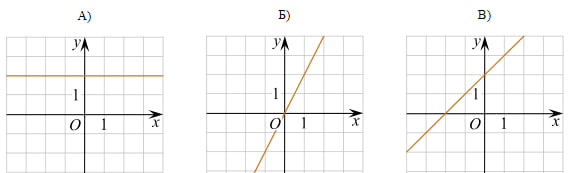
\includegraphics[align=t, width=0.8\linewidth]{../\picpath/G91M9H1}
		\end{center}
		\begin{tasks}(4)
			\task \( y=2x \)
			\task \( y=-2x \)
			\task \( y=x+2 \)
			\task \( y=2 \)
		\end{tasks}
		\item Полную механическую энергию тела (в джоулях) можно вычислить по формуле \( E=\dfrac{mv^2}{2}+mgh \),  где \( m \) --- масса тела (в килограммах), \( v \) --- его скорость (в м/с), \( h \) --- высота положения центра масс тела над произвольно выбранным нулевым уровнем (в метрах), а \( g \) --- ускорение свободного падения (в м/с\( ^2 \)). Пользуясь этой формулой, найдите \( m \) (в килограммах), если \( E=336 \) Дж,  \( v=6 \) м/с, \( h=3 \) м, а \( g=10 \) м/с\( ^2 \). 
		\item Решите неравенство: \( \dfrac{x-2}{3-x}\ge0 \)
		\item Бригада маляров красит забор длиной \( 240 \) метров, ежедневно увеличивая норму покраски на одно и то же число метров. Известно, что за первый и последний день в сумме бригада покрасила \( 60 \) метров забора. Определите, сколько дней бригада маляров красила весь забор.
		\item В равнобедренном треугольнике \( ABC \) \( AC=BC \). Найдите \( AC \), если высота \( CH=12 \), \( AB=10 \).
		\item На отрезке \( AB \) выбрана точка \( C \) так, что \( AC=75 \) и \( BC=10 \). Построена окружность с центром \( A \), проходящая через \( C \). Найдите длину отрезка касательной, проведённой из точки \( B \) к этой окружности.
		\item
		\begin{minipage}[t]{\bodywidth}
			Площадь одной клетки равна \( 1 \). Найдите площадь фигуры, изображённой на рисунке.
			\foranswer
		\end{minipage}
		\gapwidth
		\begin{minipage}[t]{\picwidth}
			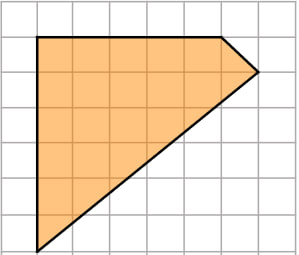
\includegraphics[align=t, width=\linewidth]{../\picpath/G91M9H1-1}
		\end{minipage}
		\item Какие из следующих утверждений верны?
		\begin{tasks}
			\task Окружность имеет бесконечно много центров симметрии.
			\task Прямая не имеет осей симметрии.
			\task Правильный пятиугольник имеет пять осей симметрии.
			\task Квадрат не имеет центра симметрии.
		\end{tasks}
	\end{listofex}
\end{homework}
%END_FOLD

%BEGIN_FOLD % ====>>_____ Занятие 3 _____<<====
\begin{class}[number=3]
	\begin{listofex}
		\item На одном из рисунков изображен график функции \(y=x^2-2x+3\). Укажите номер этого рисунка.
		\begin{center}
			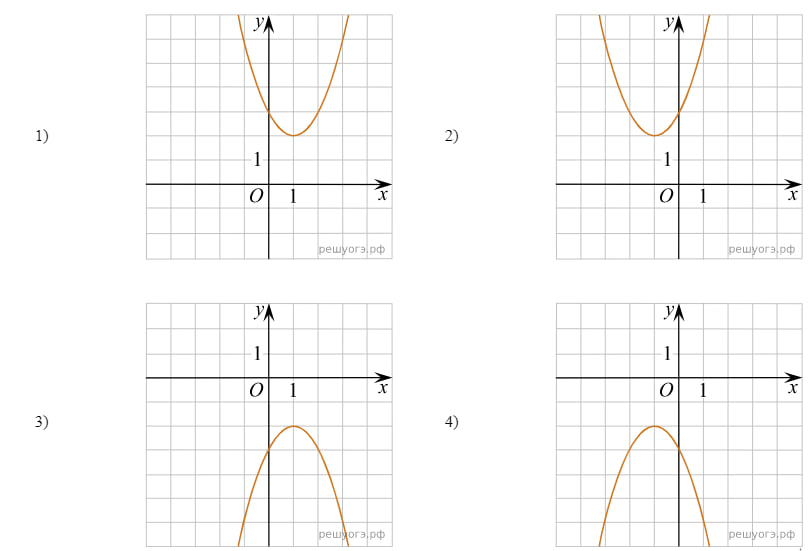
\includegraphics[align=t, width=0.8\linewidth]{../\picpath/G91M9L1}
		\end{center}
		\item Найдите значение \( k \) по графику функции y=\(\dfrac{k}{x}\),  изображенному на рисунке.
		\begin{center}
			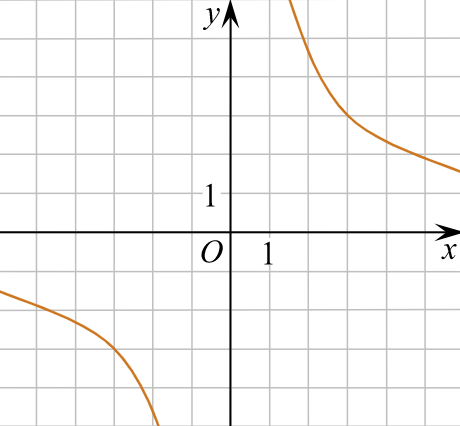
\includegraphics[align=t, width=0.3\linewidth]{../\picpath/G91M9L2}
		\end{center}
		\item Установите соответствие между графиками функций и формулами, которые их задают.
		\begin{center}
			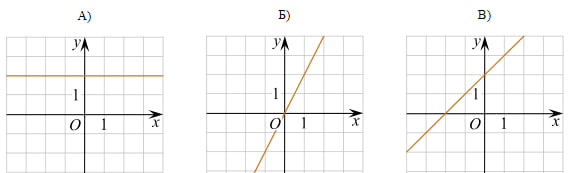
\includegraphics[align=t, width=0.8\linewidth]{../\picpath/G91M9H1}
		\end{center}
		\begin{tasks}(4)
			\task \( y=2x \)
			\task \( y=-2x \)
			\task \( y=x+2 \)
			\task \( y=2 \)
		\end{tasks}
		\item На рисунке изображены графики функций вида \(ax^2+bx+c\). Установите соответствие между графиками функций и знаками коэффициентов \(a\) и \(c\).
		\begin{center}
			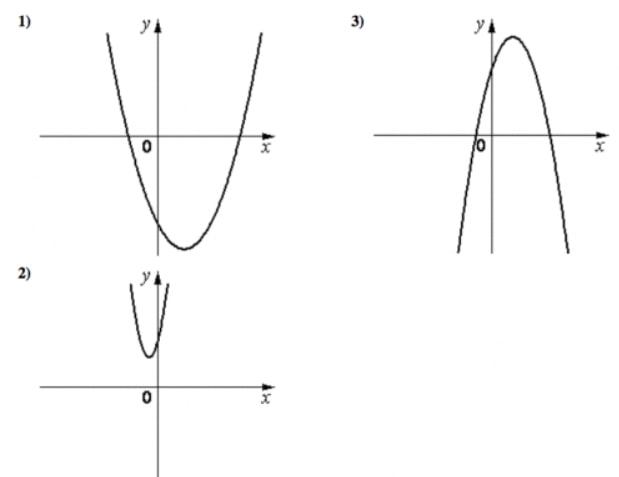
\includegraphics[align=t, width=0.7\linewidth]{../\picpath/G91M9L4}
		\end{center}
		\begin{tasks}
			\task \( a>0, c>0 \)
			\task \( a<0, c>0 \)
			\task \( a>, c<0 \)
		\end{tasks}
		\item Решите уравнение: \( \dfrac{2x^2+3x-2}{x^2-4}=1 \)
		\item Решите уравнения:
		\begin{tasks}(2)
			\task \( x^2-2x+\sqrt{3-x}=\sqrt{3-x}+8 \)
			\task \( x^2-3x+\sqrt{6-x}=\sqrt{6-x}+28 \)
		\end{tasks}
		\item Решите уравнение:
		\[x^6=(6x-5)^3\]
	\end{listofex}
\end{class}
%END_FOLD

%BEGIN_FOLD % ====>>_____ Занятие 4 _____<<====
\begin{class}[number=4]
	\begin{listofex}
		\item .
	\end{listofex}
\end{class}
%END_FOLD

%BEGIN_FOLD % ====>>_ Домашняя работа 2 _<<====
\begin{homework}[number=2]
	\begin{listofex}
		\item График какой из приведенных ниже функций изображен на рисунке?
		\begin{center}
			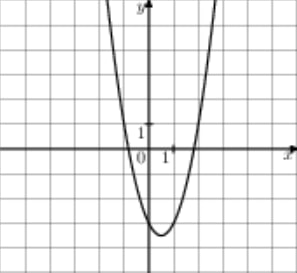
\includegraphics[align=t, width=0.4\linewidth]{../\picpath/simonovM9H2}
		\end{center}
		\begin{tasks}(2)
			\task \( y=-2x^2-2x+3 \)
			\task \( y=-2x^2+2x+3 \)
			\task \( y=2x^2+2+x-3 \)
			\task \( y=2x^2-2x-3 \)
		\end{tasks}
		\item Найдите значение \( k \) по графику функции \( y=\dfrac{k}{x} \)  изображенному на рисунке.
		\begin{center}
			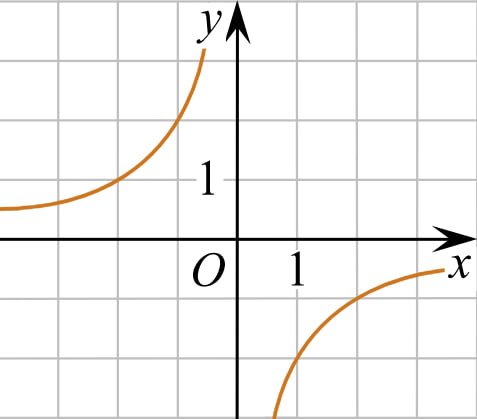
\includegraphics[align=t, width=0.4\linewidth]{../\picpath/simonovM9H2-1}
		\end{center}
		\item Решите уравнения:
		\begin{tasks}(2)
			\task \( x^6=(5x-6)^3 \)
			\task \( \dfrac{2x^2+7x-4}{x^2-16}=1 \)
			\task! \( x^2-2x+\sqrt{6-x}=\sqrt{6-x}+35 \)
		\end{tasks}
	\end{listofex}
\end{homework}
%END_FOLD

%BEGIN_FOLD % ====>>_____ Занятие 5 _____<<====
\begin{class}[number=5]
	\begin{listofex}
		\item Занятие 5
	\end{listofex}
\end{class}
%END_FOLD

%BEGIN_FOLD % ====>>_____ Занятие 6 _____<<====
\begin{class}[number=6]
	\begin{listofex}
		\item Занятие 6
	\end{listofex}
\end{class}
%END_FOLD

%BEGIN_FOLD % ====>>_ Домашняя работа 4 _<<====
\begin{homework}[number=4]
	\begin{listofex}
		\item .
	\end{listofex}
\end{homework}
%END_FOLD

%BEGIN_FOLD % ====>>_____ Занятие 7 _____<<====
\begin{class}[number=7]
	\title{Подготовка к проверочной}
	\begin{listofex}
		\item Занятие 7
	\end{listofex}
\end{class}
%END_FOLD

%BEGIN_FOLD % ====>>_ Проверочная работа _<<====
\begin{exam}
	\begin{listofex}
		\item Проверочная
	\end{listofex}
\end{exam}
%END_FOLD